\documentclass{diploma}

\student{Волков Матвей Андреевич}
\group{М8О-407Б-19}
\theme{Сервис поиска, классификации и обработки тематических изображений в интернете}

\supervisor{Филимонов Николай Сергеевич}
\firstConsultant{---}
\secondConsultant{---}
\reviewer{---}

\faculty{№ 8 <<Компьютерные науки и прикладная математика>>}
\department{806}
\speciality{01.02.03 <<Прикладная математика и информатика>>}
\profile{Информатика}

% Здесь необходим разрыв строки из-за особенностей титульной страницы
\departmentFullName{№ 806 }
\headOfDepartment{Крылов Сергей Сергеевич}

% Дата. Оставляем пустое место для дня
\date{\uline{\hspace{24pt}} мая \the\year\ года}

\newacronym{cd}{CD}{compact disk}

\newglossaryentry{id1}{ % Нужны разные id, можно ставить просто последовательно
    name={\LaTeX},
    description={система компьютерной вёрстки} 
}
\newglossaryentry{id2}{
    name={МАИ},
    description={Московский Авиационный Институт} 
}
\newglossaryentry{id3}{
    name={$S^{2}$},
    description={формула в списке обозначений} 
}

\makeglossaries
\glsaddall

\addbibresource{main.bib}

% Иллюстрации всегда по центру
\makeatletter
\g@addto@macro\@floatboxreset\centering
\makeatother

\begin{document}
    \maketitle

    % \includepdf[pages=-]{extra/task} % Задание
    \setcounter{page}{2} % Устанавливает счётчик страниц

    \abstract % Структурный элемент: РЕФЕРАТ

\keywords{КЛЮЧЕВЫЕ СЛОВА, КЛЮЧЕВЫЕ СЛОВА, КЛЮЧЕВЫЕ СЛОВА, КЛЮЧЕВЫЕ СЛОВА, КЛЮЧЕВЫЕ СЛОВА}

С другой стороны рамки и место обучения кадров представляет собой 
интересный эксперимент проверки существенных финансовых и административных 
условий. Товарищи! сложившаяся структура организации позволяет выполнять важные 
задания по разработке существенных финансовых и административных условий. 
Таким образом укрепление и развитие структуры способствует подготовки и 
реализации дальнейших направлений развития. Таким образом укрепление и 
развитие структуры способствует подготовки и реализации соответствующий 
условий активизации.

Не следует, однако забывать, что постоянный количественный рост 
и сфера нашей активности обеспечивает широкому кругу (специалистов) участие 
в формировании позиций, занимаемых участниками в отношении поставленных задач. 
С другой стороны новая модель организационной деятельности требуют определения 
и уточнения систем массового участия. Не следует, однако забывать, что 
постоянное информационно-пропагандистское обеспечение нашей деятельности 
представляет собой интересный эксперимент проверки позиций, занимаемых 
участниками в отношении поставленных задач. Задача организации, в особенности 
же реализация намеченных плановых заданий требуют от нас анализа существенных 
финансовых и административных условий. % Реферат

    \tableofcontents % Содержание 
    \termsanddefenitions % Термины и определения
    \listofabbreviations % Перечень сокращений и обозначений
 
    \introduction % Структурный элемент: ВВЕДЕНИЕ

В данном документе описываются основные моменты работы с шаблоном. Приведены примеры ко всему, что может понадобится при написании отчета, даны пояснения касаемо особенностей оформления. Вопросы содержания не рассматриваются, обращайтесь к шаблону, предоставленному институтом (ссылка в README).

Цитирование источника 1 \cite{Wikipedia1}.
 % Введение

    % Название разделов -- все прописные
\section{ТЕОРЕТИЧЕСКАЯ ЧАСТЬ}

\subsection{Обоснование библиотек}

В микросервисе были использованы внешние модули для упрощения частоиспользуемых действий в коде.
Каждая из них представляет собой очень полезную функциональность, которая будет перечислена ниже с обоснованием использования.

\subsubsection{pdfcpu}
Pdfcpu \cite{pdfcpu-cite} --- пакет, написанный на ЯП GO, яляющийся мощным сборником pdf файлов. Представляет интферфейс для создания сложноструктурированных pdf файлов.

В данном пакете возможно создавать абсолютно любые pdf файлы с различными метаданными документа, начиная с содержания, заканчивая указыванием автора написания документа.
Библиотека способна также использовать различные картинки различных разрешений, позволяя менять их размер, цвет, прозрачность и другие параметры.

Пакет был взят в использование потому, что предоставляется разработчиками удобный и понятный интферфейс для собирания большого количество картинок в pdf файл. 
Также модуль отличается своей быстротой исполнения поставленных задач. Рисунок~\ref{libs-pdfcpu} может продемонстрировать простоту использования пакета.

\begin{figure}
\begin{lstlisting}[language=go]
func CreatePDFFromImagesDir(imagesDirPath string, outputPath string) error {
	imagesPath, err := GetImagesPathStr(imagesDirPath)
	if err != nil {
		return errors.Wrap(err, "something wrong with creating images path")
	}
	err = api.ImportImagesFile(imagesPath, outputPath, nil, nil)
	if err != nil {
		return errors.Wrap(err, "pdf creation filure")
	}
	return nil
}
\end{lstlisting}
\caption{Демонстрация работы интерфейса pdfcpu}
\label{libs-pdfcpu}
\end{figure}


\subsubsection{goquery}
Goquery \cite{goquery-cite} --- пакет, написанный на ЯП GO, который способен выполнять задачи библиотеки jQuery \cite{jquery-cite}. 

Данный пакет используется для того, чтобы парсить DOM дерево полученного HTML файла. С ним возможно быстро и удобно получить нужную информацию с любого сайта.
После реверс-инженеринга, благодаря этому покету, быстро и просто достается информация о картинках, классифицируется на разделы и подразделы (например, группировка на главы).

\begin{figure}
	\begin{lstlisting}[language=go]
	func (mlb mangaLibController) getChapterID(doc *goquery.Document) (string, error) {
		result, ok := doc.Find("#comments").Attr("data-post-id")
		if !ok {
			return "", errors.Wrap(customerrors.ErrEmptyAttr, "mangalib: data-post-id")
		}
		return result, nil
	}
	\end{lstlisting}
	\caption{Демонстрация работы пакета goquery}
	\label{libs-goquery}
\end{figure}

Как видно из рисунка~\ref{libs-goquery}, видно, что используются команды jQuery для получения информации о главе. Далее эта глава используется дальше, чтобы достать картинки этой главы.

\subsubsection{jet}
Go-jet \cite{jet-cite} --- пакет, написанный на ЯП GO, являющийся конструктором SQL запросов в БД.

С помощью этой библиотеки возможно собирать любые SQL запросы, избегая уязвимость --- SQL-инъекцию. 
Этот пакет подключается к БД и генерирует код на языке GO, при помощи которого можно собирать различные SQL запросы.
От инъекции помогает избавиться тот факт, что абсолютно весь запрос делается при помощи конструктора, в процессе сбора которого есть постоянные проверки на соответствие данных,
поступающих в процесс создания запроса.
Также стоит заметить, что сама возможность собирать запрос из различных кусочков, может очень сильно помочь при составлении денамического запроса, который так или иначе зависит от поступивших на вход параметров.

Именно по этой причине был выбран данный пакет.
Как можно видеть из рисунка~\ref{libs-jet}, собирается SQL запрос в зависимости от пришедших на вход параметров. 
Таким образом, условная секция запроса может варьироваться.

\begin{figure}
	\begin{lstlisting}[language=go]
		func (perC personController) GetEmailByID(ctx context.Context, person domain.PersonInfo) (string, error){
			selectStmt := table.Persons.SELECT(table.Persons.Email)
			var whereStmt postgres.BoolExpression
		
			personID, _ := uuid.Parse(person.PersonID)
			switch {
			case personID != uuid.UUID{} && personID != uuid.Nil:
				whereStmt = table.Persons.ID.EQ(postgres.UUID(personID))
			case person.TelegramID > 0:
				whereStmt = table.Persons.TelegramID.EQ(postgres.Int64(person.TelegramID))
			default:
				return "", customerrors.ErrEmailsNotFound
			}
			stmt, args := selectStmt.WHERE(whereStmt).Sql()
		
			...
		
			return email, nil
		}
	\end{lstlisting}
	\caption{Демонстрация работы пакета jet}
	\label{libs-jet}
\end{figure}


\subsection{Устройство сайтов}
Предметом исследования диплома был ограниченный список сайтов,
участвующие в сборе картинок с последующей их сортировкой и группировкой в pdf файл для последующего их удобного просмотра или прочтения.
Суть изучения состояло в том, чтобы произвести реверс-инженеринг сайта, понять как он работает. 
Затем использовать полученные знания в поиске нужной мне информации, путем парсинга страницы сайта, разбиения полученной структуры сайта на составляющие,
с последующей структуризацией в нужный мне формат для правильной отдачи итогого результата.

Абсолютно любой сайт состоит из 3-х компонент:

\begin{enumerate}
    \item HTML
    \item CSS
    \item JavaScript
\end{enumerate}  

\subsubsection{HTML}
В данной компоненте описывается различная информация о странице. Будь то текст статьи, картинки и прочее.
Затем, браузер, применяя свои движки визуализации, преображает инфорацию, содержащуюся в компоненте, в понятную для человека визуализированное представление.
HTML имеет свою структуру, называемой DOM деревом. Эта структура по сути своей является набором различных тэгов.
Для идеального примера можно сказать, что HTML похож на LATEX. Таким образом, HTML --- это то, откуда будет получаться нужная информация.

Как было сказано ранее, HTML состоит из тэгов. Есть следующие виды тэгов:
\begin{enumerate}
    \item Двойные
    \item Ординарные
\end{enumerate} 

Двойной тэг отличается от ординарного тем, что у двойного тэга есть закрывающий тэг. Между открывающим тэгом и закрывающим пишется текстовая информация.
Например, на рисунке~\ref{html-tag-2} продемонстрирован двойной тэг, обозначающий параграф. Обычно такой тэг используется в различных статьях.
На рисунке~\ref{html-tag-1} продемонстрирован пример ординарного тэга, обозначающий картинку. Когда браузер видит этот тэг, он понимает, что перед ним картинка.
За кадром происходит запрос на сервер по ссылке, расположенной в мета информации, с последующим отображением изображения.

\begin{figure}
    \begin{lstlisting}[language=html]
        <p class="paragraf">Текст параграфа</p>
    \end{lstlisting}
    \caption{Пример двойного тэга}
    \label{html-tag-2}
\end{figure}
\begin{figure}
    \begin{lstlisting}[language=html]
        <img src="picture.img" alt="Cup of Kitty">
    \end{lstlisting}
    \caption{Пример ординарного тэга}
    \label{html-tag-1}
\end{figure}

На картинках \ref{html-tag-2} и \ref{html-tag-1} были продемонстрированы тэги, которые требуют от браузера некоторых действий.
Но, как было выше отмечено, HTML очень похож на LATEX. И похож он тем, что в основном страницы сайта нужно верстать. 
Поэтому люди придумали тэг, который не требует никаких действий со стороны браузера, но при этом будет как-то объединять информацию.

На рисунке~\ref{html-div} изображен тэг div. Этот тэг нужен исключительно для того, чтобы как-то объединять информацию, присваивая ей какую-то общую метаинформацию, например, класс.

\begin{figure}
	\begin{lstlisting}[language=html]
	<div class="pritty"></div>
	\end{lstlisting}
	\caption{Тэг div}
	\label{html-div}
\end{figure}

Из совокупности тэгов состоит страница сайта. А структура, которая в конечном итоге образуется, называется DOM деревом.

\subsubsection{CSS}
Эта компонента, в свою очередь, отвечает за то как будет выглядить информация, содержащаяся в HTML. По сути своей, CSS --- оформление страницы.
После появления данной компоненты, сайты в интернете стали выглядить так, как мы их сейчас видим.

Для формирования различных стилей, используется метаинформация тэгов. 
Удобнее всего для таких нужд оказалось использовать тэг, изображенный на рисунке~\ref{html-div}, так как этот тэг как никто лучше служит для объединения информации, которую можно как-то по-особенному
расположить и украсить.

Именно поэтому на большинстве сайтов можно увидеть именно этот тэг.

\subsubsection{JavaScript} \label{js-ref}
Эта компонента отвечает за логику на страницах. Логика может использоваться при анимировании сайтов и общения с сервером. Общение с сервером нужно для того, чтобы возможно было у него получить какую-то информацию.


 

\subsection{Методика парсинга}
Понимание сайта --- важная часть абсолютно любого парсинга данных. Как понятно из определения, необходимо собирать информацию.
Для того, чтобы собирать информацию, необходимо знать как она расположена.
Для того, чтобы понимать как расположена информация, необходимо исселодовать пути появления этой информации перед пользователем и 
выяснить откуда она берется.

Плавно мы подбираемся к тому, что знание устройства сайта, клиентской части и сервера --- необходимы для ранее сказанного парсинга данных.
Другими словами, для парсинга данных с сайта необходимо полностью понимать как тот устроен. 
Если же не получается полностью изучить, то необходимо понять, какие данные должны использоваться, чтобы в конечном итоге достичь нужного результата.
Нужно цепляться буквально за любую крупицу данных, которая может так или иначе помочь.

\subsubsection{Взаимодействие с сервером}
Для поиска подобной крупицы информации нужно понимать, что ничего не происходит из ниоткуда. Везде есть какие-то следы.
Они могут быть зашифрованы, или спрятаны за тонной других запросов. Но информация откуда-то получается.
Нужно сделать оговорку, потому что есть сайты, которые не используют сервер для получения какой-либо информации, 
а она уже сразу закодирована в верстке сайта. Такими сайтами называются <<визиткой>>.
Как понятно из навзвания, такие сайты нужны для того, чтобы красиво продемонстрировать род деятильности, прорекламировать компанию,
которую представляет тот или иной сотрудник и указать там контакты для сотрудничества.
Обычно такие сайты одностроничные, под собой не имеют никакой логики. Такие сайты очень удобно парсить.
Но чаще всего человек сталкивается с сложными сайтами со сложной логикой, где есть большая база пользователей и контета.
Такие сайты просто обязаны обращаться за какой-то логикой на сервер.

Можно заметить, что в разделе \ref{js-ref} упоминается JS --- логическая сторона сайта. Почему не пользоваться этой замечательной компонетой сайта для различной логики?
Дело, конечно же, в безопасности. Куда более надежно будет положить какую-то информацию в переменную, а потом ее в будущем отобразить на странице при помощи, например, jQuery.
Никто не хочет, чтобы алгоритмы обработки личной информации лежали перед всеми на видном месте, чтобы их можно было запустить и все расшифровать.
Или как еще по-другому можно хранить миллионы миллиардов информации?

Итак, так как предмет исследования как раз идет за нужной информацией на сервер, 
необходимо понять из каких крупиц информации создаются следующие более сложные запросы на сервер.
Для этого необходимо изучить выдаваемую информацию на сайте, запросы, которые исполняются в процессе загрузки страницы.
Исследование нужно производить с конца, идя в самое начало.
Например, если мне нужно достать нужную мне картинку, то мне нужно найти запрос, который эту картинку запрашивает.
Далее нужно найти запрос, который делает предыдущий запрос и так до самого основание.

Таким образом мы можем понять как сайт взаимодействует с сервером при различном получении разных страниц.

\subsubsection{Изучение данных}
Необходимо сделать несколько оговорок:
\begin{itemize}
    \item все примеры будут продемонстрированы в браузере Google Chrome, так как в нём имеется богатый инструментарий для программистов, а также поддерживается огромное колличество сайтов, ведь именно этот браузер является самым популярным \cite{broser-popularity-cite},
    \item комбинации клавиш, продемонстрированные в примерах, актуальны для операционной системы Windows.
\end{itemize}

Для поиска информации необходимо пользоваться инструментом разработчика. Открывается данное меню разработчика при помощи нажатия клавиши F12. 
На рисунке~\ref{chrome-tools-pic} продемонстрировано меню.

\begin{figure}
    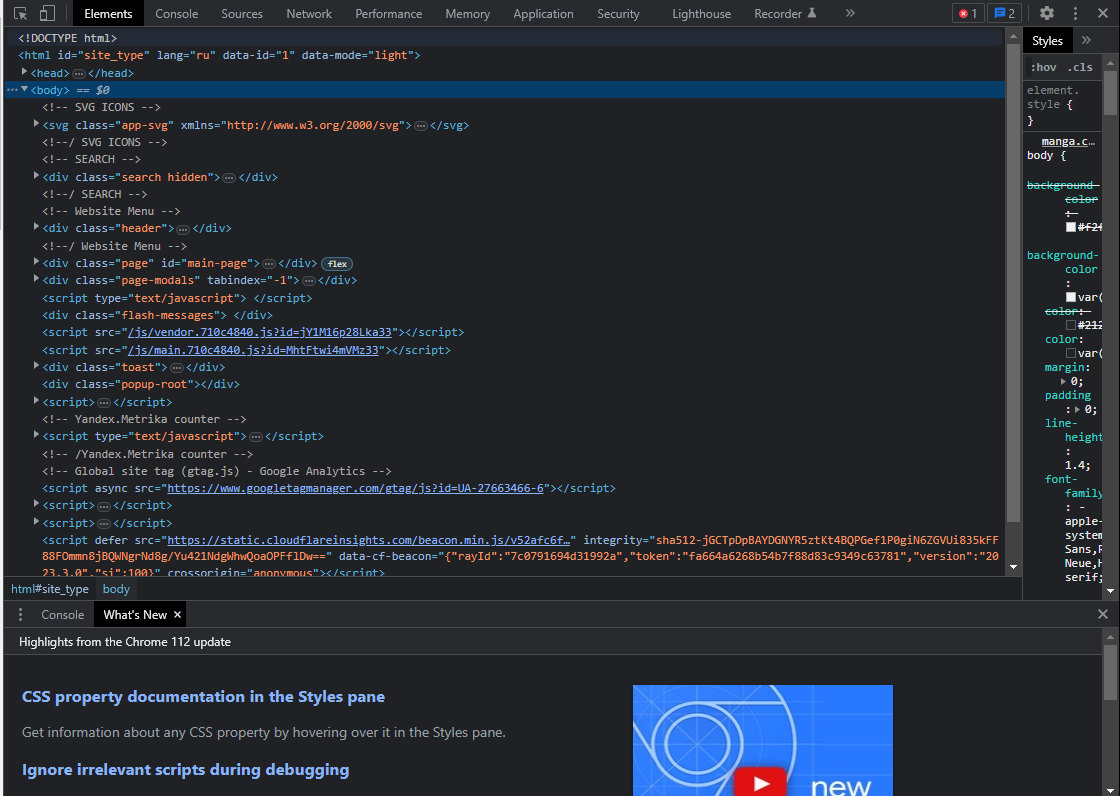
\includegraphics[scale=0.5]{imgs/chrome-tools}
    \caption{Меню разработчика}
    \label{chrome-tools-pic}
\end{figure}

У браузера есть свойство, при котором он исполняет все скрипты в тегах языка HTML. 
Как говорилось ранее, эти скрипты могут содержать запросы на сервер за получением информации на страницу.
Также еще нужно знать, что вписывание ссылки в браузер и последующем нажиманием подтверждения ввода, по сути своей делает GET запрос на домен с соответствующим роутингом.
Зная также тот факт, что на один запрос приходится один ответ, мы можем определенно точно сказать, что программа наша получит сайт с первичной информацией. 
То есть будет загружены скрипты, которые делают последующие запросы на сервер.
Из этого мы можем сделать вывод, что просто так никакая информация из ниоткуда не берется и с большой вероятностью мы при помощи только одного запроса не получим весь сайт. 
Для тестирования запросов можно пользоваться удобным инструментом postman \cite{postman-cite}.
На рисунке~\ref{postman-first-get} продемонстрирован пример одного GET запроса на сайт через инструмент postman. 
На рисунке~\ref{html-add} приложения изображена команда, которую можно сделать, чтобы посмотреть полностью код HTML.

\begin{figure}
    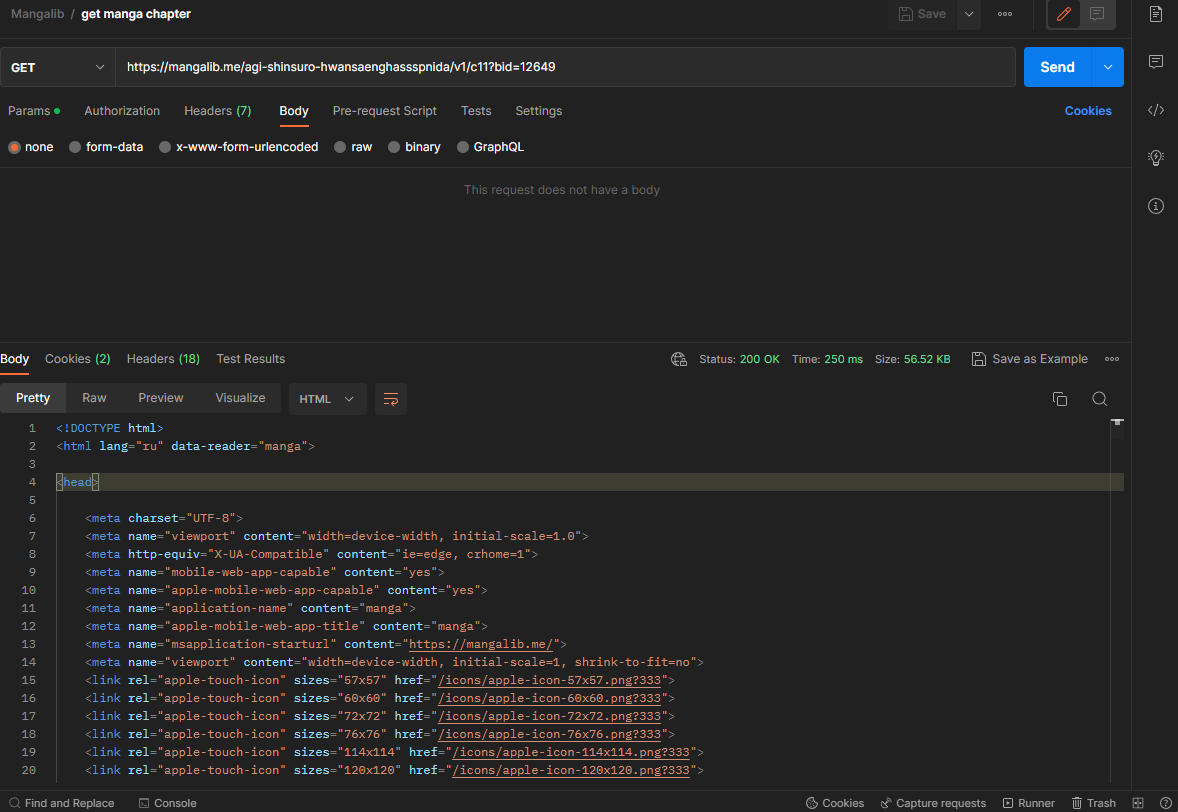
\includegraphics[scale=0.5]{imgs/postman-get-site}
    \caption{GET запрос }
    \label{postman-first-get}
\end{figure}

Из кода можно увидеть, что HTML код очень сильно отличается от того, что изображен в меню разработчика.
Это все потому, что мы не проделали все те запросы, что делает браузер, когда начинает прогрузку страницы.
К счастью, нам этого делать не надо. Это лишь доказательство того, что до любой информации мы можем одним или несколькими путями добраться.

Для того, чтобы начать изучение данных, необходимо зайти на сайт и найти самостоятельно ту конечную информацию, которая нужна. 
В данном случае ведется поиск картинок.
После того, как мы нашли нужную картинку, необходимо понять как выглядит ссылка на нее.
Исходя из той логики, что разработчик сайта будет составлять ссылку из абсолютно случайного набора букв и цифр -- крайне мала, так как это решение бесполезно и очень сильно влияет на быстроту разботки в худшую сторону,
мы можем попробовать догадаться по какой логике конструируется ссылка на ресурс. Итак, чтобы посмотреть на ссылку картини, нам необходимо посмотреть код этой картинки в HTML.
На рисунке~\ref{chrome-tools-image-tag-pic} видно, как выделен тэг картинки, которую мы бы хотели получить. 

\begin{figure}
    
\includegraphics[scale=0.5]{imgs/chrome-tools-image-tag}
    \caption{Представление картинки в кода HTML}
    \label{chrome-tools-image-tag-pic}
\end{figure}

Посмотрев так на другие картинки, можно увидеть, что у них у всех есть один источник.
А ссылка формируется по паттерну из рисунка~\ref{image-pattern-add}. Следовательно возможно эту ссылку конфигурировать своими руками в сервисе.
Для этого нам нужны:

\begin{itemize}
    \item название манги,
    \item правильных id главы,
    \item хеш картинки.
\end{itemize}

Теперь необходимо узнать где на странице еще лежит вышеописанная информация. Для этого нам нужно проанализировать запросы.
Для этого нам пригодится вкладка Network в меню разработчика.
На странице картинки открываем меню разработчика и перезагружаем страницу.
Это нужно для того, чтобы во вкладке появились все абсолютно запросы, которые делает браузер для того, чтобы прогрузить полностью страницу.
На рисунке~\ref{chrome-tools-network} продемонстрирован весь список запросов, который делается при загрузке страницы определенного сайта.
Очевидно этот список может отличаться от того, что продемонстрировано на рисунке~\ref{chrome-tools-network}.

\begin{figure}
    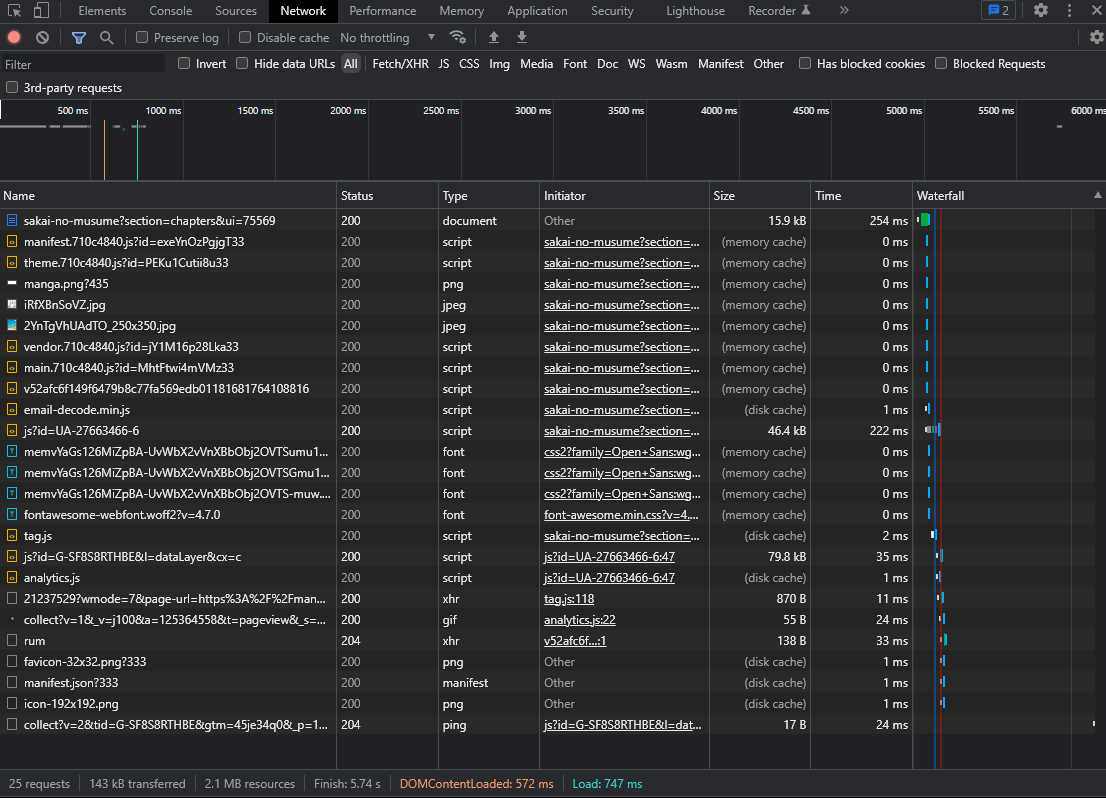
\includegraphics[scale=0.5]{imgs/network-example}
    \caption{Меню разработчика network вкладка}
    \label{chrome-tools-network}
\end{figure}

Далее необходимо найти эту картинку в запросах. В меню есть фильтр по типам файлов. Выбираем там картинки.
На рисунке~\ref{chrome-tools-network-pics} мы видим, что не очень много запросов было на картинки.
С легкостью можем найти наш файлик (на рисунке выделен).
Можно еще также заметить, что разработчики постарались и заренее прогружают следующую страницу, чтобы было проще смотреть контент.

\begin{figure}
    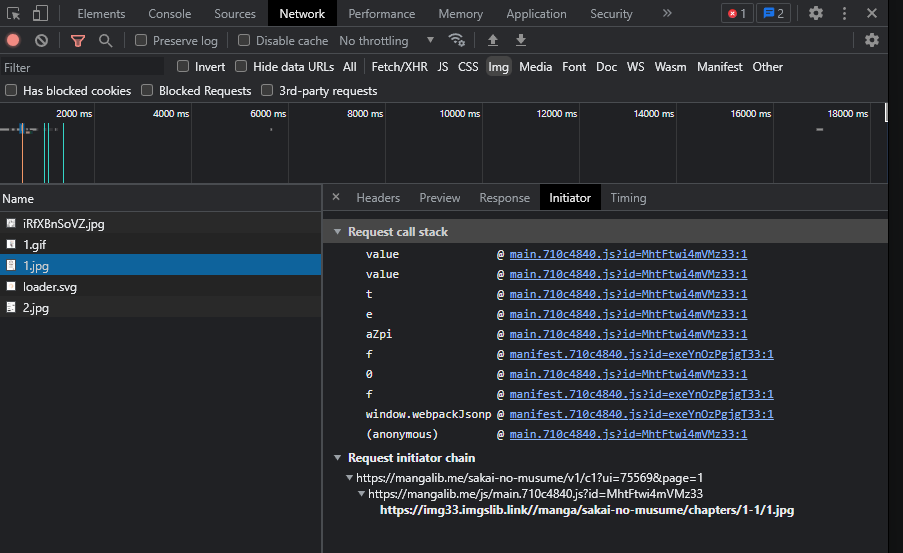
\includegraphics[scale=0.5]{imgs/network-pics}
    \caption{Меню разработчика network вкладка с фильтром по картинкам}
    \label{chrome-tools-network-pics}
\end{figure}


Теперь нам необходимо узнать как был получен запрос на эту картинку. 
Помним, что из-за особенности устройства браузера информация не появляется из ниоткуда.
Следовательно мы можем с легкостью узнать откуда пришел запрос.
Благо нам не нужно особо много, чтобы раздобыть подобного рода информацию.
Меню разработчика предоставляет интерфейс для показа стека вызова. На рисунке~\ref{chrome-tools-network-pics} можно увидеть вкладку Initiator.
Это и есть наш стэк вызовов.

На самом деле, если мы будем смотреть код каждого запроса, сможем легко закопаться в нем, так как чаще всего подобного рода сайты подключают разные сервисы для генерации логики.
Этот сайт не исключение. Здесь добавлена защита от DDOS атак от компании Яндекс, также трекер использования сайта.
Через подобного рода скрипты происходит процесс анализа запросов. Поэтому в середине запроса может быть сгенерированный код, который почти невозможно понять без нескольких дней его анализа.
Благо в нашем случае его анализировать не надо.
Можно начать смотреть код, который находится вокруг места, откуда произошел вызов того или иного запроса.
Таким образом натыкаемся на самый первый вызов в стеке и замечаем, что это наш любимый HTML код.
Изучив его, можно увидеть, что есть большой скрипт. В нем есть переменная <<window.\_\_DATA\_\_>> (при помощи вызова скрипта на рисунке~\ref{html-add} можно увидеть этот скриат).
Кажется это то, что нам нужно.

Переменная <<window.\_\_DATA\_\_>> --- JSON, в котором явно написана информация о манге.
Исследовав этот объект, обнаруживаем, что там есть информация о названиях каждой страницы. Можно также ваявить и сколько страниц в данной конкретной главе.
На рисунке~\ref{json-structs-parsing} можно посмотреть на получившуюся структуру, в которую можно парсить из JSON.

\begin{figure}
	\begin{lstlisting}[language=go]
		type pageList struct {
            Page int    `json:"p"`
            Url  string `json:"u"`
        }
	\end{lstlisting}
	\caption{Структры содержания информации о главах и картинках}
	\label{json-structs-parsing}
\end{figure}

В Url атрибуте хранится тот самый хэш картинки.
ID главы можно узнать из атрибутов на той же странице.
Название манги совсем просто найти. Оно находится буквально в каждой ссылке данного сайта. Поэтому можно просто скопировать название оттуда.

Примеры выше были для сайта mangalib.me, участвующий в итоговом дипломе.
Анализ каждого сайта происходит в индивидуальном порядке, так как везде свои разные алгоритмы и подходы.
Задача микросервиса сделать так, чтобы добавление новых сайтов было достаточно простым и требовало исключительно анализа и исполнении всех алгоритмов для автоматического поиска.


\subsubsection{Сайты с API}
Есть некоторые сайты, разработчики которых подумали о пользователях и о том, что эти пользователи возможно хотели бы автоматизировать процесс поиска и скачивания контента.
Одним из таких сайтов является mangadex \cite{mangadex-cite}.

Для подобных сайтов нет необходимости заниматься реверс-инженерингом, как было представлено выше. 
Достаточно изучить документацию \cite{mangadex-api-cite} и найти хендлеры, которые выполняют поставленную задачу и использовать их.
Однако, это не означает, что предварительную обработку не нужно делать.
Благо вышесказанный сайт имеет много примеров использования и свой SWAGGER \cite{swagger-cite} для тестирования.

Тестирование подобного API происходит через принцип <<проб и ошибок>>, так как не всегда случается такое, что появляется на выходе ожидаемая информация.
В некоторых случаях нужно заниматься ее обработкой.
\subsection{База данных в микросервисах}
Для некоторых микросервиов база данных совсем не нужна.
Такие микросервисы обычно не используют никакую информацию, например, сервисы по конвертированию данных.
Там запускается какой-то разовый алгоритм и все.
Часто сохранять информацию в один csv файл.
Однако сервисы, которые в основе своей работают с данными пользователями, просто необходим.
Собранную информацию потом возможно использовать для анализа, чтобы, например, делать на ее основе модели искусственного интеллекта.

Одной из основных причин использования баз данных в микросервисах является возможность распределения данных и обработки запросов между несколькими сервисами.
Каждый сервис может иметь свою собственную базу данных или использовать общую базу данных, что позволяет сократить нагрузку на каждый сервис и повысить производительность всей системы.

Кроме того, базы данных обеспечивают целостность данных и защиту от потери информации. 
Они позволяют хранить информацию в структурированном виде, что упрощает ее поиск и обработку.
Базы данных также обеспечивают безопасность данных, позволяя контролировать доступ к ним и устанавливать права доступа для каждого сервиса.

Базы данных также позволяют решать проблемы масштабирования и управления ресурсами. 
Благодаря возможности горизонтального масштабирования баз данных, можно легко расширять хранение данных и увеличивать производительность системы при необходимости. 
Кроме того, базы данных позволяют эффективно управлять ресурсами, например, памятью и дисковым пространством, что повышает эффективность работы всей системы.

Использование баз данных в микросервисах также упрощает разработку и тестирование сервисов. 
Каждый сервис может использовать свою собственную базу данных для тестирования и разработки, что позволяет избежать конфликтов между сервисами и обеспечить более быстрое и эффективное тестирование.

Также, базы данных помогают поддерживать констистентность данных. Очень важно эту особенность учитывать и в сервисе по поиску картинок.
На ее основе можно сохранять ранее полученную информацию и не беспокоить сайт при каждом новом запросе.
Эта особенность очень важна в тех случаях, если сайт имеет защиту против DDOS атак.
Если сервисом будет пользоваться даже сотни людей, то у сайта может возникнуть вопрос о появлении стольких запросов с одного IP.
Именно поэтому намного лучше и проще будет сохранять всю информацию в базе данных.

Приведу пример, есть популярная манга, которая так или иначе пользуется спросом.
При помощи поиска этой же манги и конкретной главы возможно сразу из памяти БД достать информацию, лишний раз не нагружая сайт запросами.
Таким образом такое поведение очень хорошо скажется на:
\begin{enumerate}
    \item работоспособности приложения. Не придется каждый раз ждать ответа от конкретного сайта.
    \item внезапно не будет заблокирован наш микросервис за большое количество запросов на сайт
    \item не придется в микросервисе обходить защиту от роботов (captcha)
\end{enumerate} 

Перед тем, как использовать БД, нужно также подумать о том что будет храниться там. Очень важно это сделать на этапе конструирования.
Иначе может получиться так, что эффекта от такого мощного инструмента не будет.

Также при помощи БД возможно сделать подписку на обновление контента. С ее помощью можно организовать рассылку, достав большой объем нужных данных.
С файлом csv это было бы очень трудно сделать.

Также преимуществом работы с БД является транзакции.
При помощи транзакции можно изменять чувствительные данные, не боясь при этом гонки (race condition).
\subsection{Чистая архитектура} \label{clean-arch}
Clean Architecture - это популярный подход к разработке программного обеспечения, 
который был предложен Робертом Мартином (также известным как Uncle Bob). 
Этот подход помогает разработчикам создавать гибкие, расширяемые и легко тестируемые приложения.

В Golang Clean Architecture часто реализуется с помощью пакетов и интерфейсов. 
Пакеты используются для организации кода в логически связанные блоки, 
а интерфейсы - для определения контрактов между различными компонентами приложения.
На рисунке~\ref{clean-arch-pic} представлена схема такого взаимодействия пакетов.

\begin{figure}
    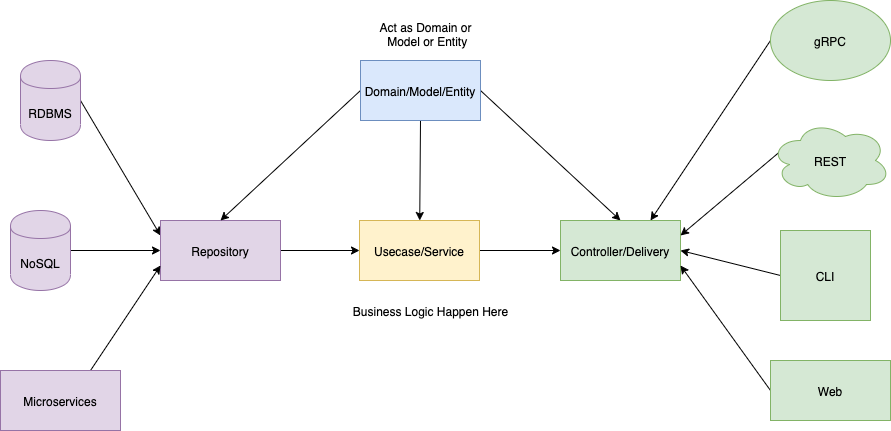
\includegraphics[scale=0.5]{imgs/clean-arch}
    \caption{Схема чистой архитектуры}
    \label{clean-arch-pic}
\end{figure}

В центре Clean Architecture находится принцип разделения зависимостей (Dependency Inversion Principle), который гласит, что зависимости должны быть направлены от абстракций к конкретным реализациям, а не наоборот.
Это позволяет разработчикам легко заменять реализации компонентов приложения, не затрагивая другие части системы.
Так, например, область, отвечающая за сохранение данных не должна содержать никакую логику.
Она должна только выдавать или сохранять данные.

Стоит оговориться, что не стоит обязательно точно придерживаться этому концепту.
Иногда в этом нет особой надобности.
Но такое разделение лучше делать всегда и сохранять его в том или ином виде.

Одним из основных преимуществ Clean Architecture в Golang является возможность легко тестировать каждый слой независимо от других. 
Это достигается путем использования интерфейсов для определения контрактов между слоями. 
Это позволяет разработчикам легко заменять реализации компонентов приложения на макеты (mocks) для тестирования.

Кроме того, Golang Clean Architecture обеспечивает высокую гибкость и расширяемость приложения. 
Благодаря разделению зависимостей и использованию интерфейсов, программисты могут легко добавлять новые функции и изменять существующие, не затрагивая другие части системы.

В Golang Clean Architecture используется многослойная архитектура.

\subsubsection{Представление (Presentation Layer)}
Этот слой отвечает за взаимодействие с пользователем и обработку входящих запросов.
Он содержит контроллеры, представления и другие компоненты, которые отображают данные для пользователя.
В вышеизложенном сервисе расположены хендлеры, которые отвечают за обработку запросов по конкретному роутингу.

\subsubsection{Использование (Use Case Layer)}
Этот слой содержит бизнес-логику приложения. 
Он определяет, как приложение должно взаимодействовать с данными и какие операции должны быть выполнены. 
Он также содержит интерфейсы для доступа к данным.
Например, в этом слое можно организовать логику парсинга картинок, организацию их по подгруппам и сбор в pdf.
Затем данные отправлять в следующий слой.

\subsubsection{Хранилище (Storage Layer)}
Этот слой отвечает за хранение данных и доступ к ним. 
Он содержит реализации интерфейсов, определенных в слое использования. 
Эти реализации могут использовать различные источники данных, такие как базы данных, файлы или внешние API.

\subsubsection{Инфраструктура (Infrastructure Layer)}
Этот слой содержит код, который не относится к бизнес-логике приложения, но необходим для его работы. 
Это может быть код для обработки ошибок, логирования, аутентификации и т.д. 
Этот слой также содержит реализации интерфейсов, определенных в слое использования, для доступа к внешним сервисам и системам.

На рисунке~\ref{clean-arch-add} демонстрируется пакетное представление проекта.
 % Теоретическая часть
    \section{ПРАКТИЧЕСКОЕ ПРИМЕНЕНИЕ}

\subsection{Структура приложения}
Приложение состоит из основной серверной части --- API и клиентских частей. 
Клиентским сервисом считается любой сервис, например бот в мессенджере, способный отправлять запросы на серверную часть.
Серверная часть выполнена в соответствии с концепцией чистой архитектуре, в соотвествии с тем, что описан в рзеделе \ref{clean-arch}.
На рисунке~\ref{clean-arch-add} изображена схема проекта.
Каждый пакет отвечает за свою определенную часть.

Пакет <<repository>> отвечает за взаимодействие между БД. В <<cmd>> находится main.go файл, который запускает сервер.
<<App>> содержит в себе реализацию хендлер функций. Пакет <<config>> используется по всему проекту. 
В нем описаны функции, помогающие доставать различные секреты приложения, такие как пароли, из переменных окружения.
В этом же пакете происходит парсинг тех из yaml файла.
В пакете <<gen>> содержится сгенерированные структуры библиотекой jet из раздела \ref{jet-section}. 
В <<internal/pgk>> содержатся все пакеты, которые так или иначе выполняют какую-то логигу приложения.
Своего рода usecase слой.
Пакет <<parse>> отвечает за логику парсинга описанного для конерктного сайта. Так можно увидеть там один из объектов исследования --- сайт mangalib
<<Pdf\_creator>>, как понятно из названия, занимается описанием логики сбора картинок в один pdf файл.
Пакет <<mailer>> необходим для того, чтобы отправлять файлы через через какие-либо возможные способы передачи, например, отправки тех через электронную почту.
В папке <<migrations>> описан SQL код всех миграций БД.

Внешние пакеты (те, что находится не в папке <<internal>>) используются для того, чтобы к ним возможно было получить доступ мнешним клиентским сервисам.
Так в <<api>> пакете описаны структуры request и response, отвечающие за боди запроса и ответа соответственно.
Также в модуле описан роутинг API. 
Пакет <<pgk>> необходим для того, чтобы импортировать тот в клиентский сервис, так как там предполагается описание sdk.
В этом пакете описаны кастомные ошибки, которые можно в последствии обработать.
\subsection{БД в парсинге}
Важной составляющей микросервиса является база данных. 
В ней хранится совсем вся информация о пользователях и о структуре манги.
Главной особенностью базы в данном проекте является то, что можно контролировать количество пользователей, которые используют сервис.
Таким образом возможно принимать решение о том нужно ли заниматься оптимизацией или улучшением компонент сервера. 
БД также позволяет легко получить доступ к данным, ограничить его же другим пользователям и легко перенести информацию от одного сервера в другой.

Однако, выше были перечисленные общие преимущества для микросервисов.
Главным же преимуществом базы данных в данном проекте заключается в том, что можно сохранять структуру глав к любой манге.
Таким образом не придется делать большое количество запросов на каждого пользователя. 
Возможно ограничиться только запросами на загрузку картинок с сервера.
При использовании клиентского сервиса в виде мессенджера телеграм, возможно загружать мангу, создавая статьи.
Каждой статье в телеграме предоставляется своя ссылка. 
Так при генерировании статьи пользователем, ссылка может сохраниься в базе данных. 
В случаях, когда какая-то манга является популярной, возможно лишь выдавать в последствии ссылку уже подготовленную статью.
Преимущество статьи выражается в том, что телеграм подготовил весь необходимый удобный интерфейс. Поэтому просмотр комикса выглядит локанично.

Если к API подключить сервис по облачному хранилищу или же прямо непосредственно на сервере хранить все уже загруженные и сгенерированные главы в виде pdf, 
то вполне возможно загружать в БД пути к определенным файлам, чтобы не делать заново генерацию.

БД может помочь в дальнейшем развитии проекта, а именно организации подписки на рассылку выхода новой главы конкретной манги. 
Так можно сделать воркер, способный в фоне раз в какое-то время обновлять структуру глав манги.
При обновлении этой структуры, будет происходить рассылка пользователям, которые подписались на обновление комикса.
Структуру глав манги можно хранить в виде документа JSON.

Особенностью конструирования схемы БД является то, что обновление ее происзводится при помощи миграций \cite{migrations-cite}.

\subsubsection{Описание сущностей БД}
На рисунке~\ref{db-struct-pic} представлена схема БД, которая используется на момент написания ВКР.

\begin{figure}
    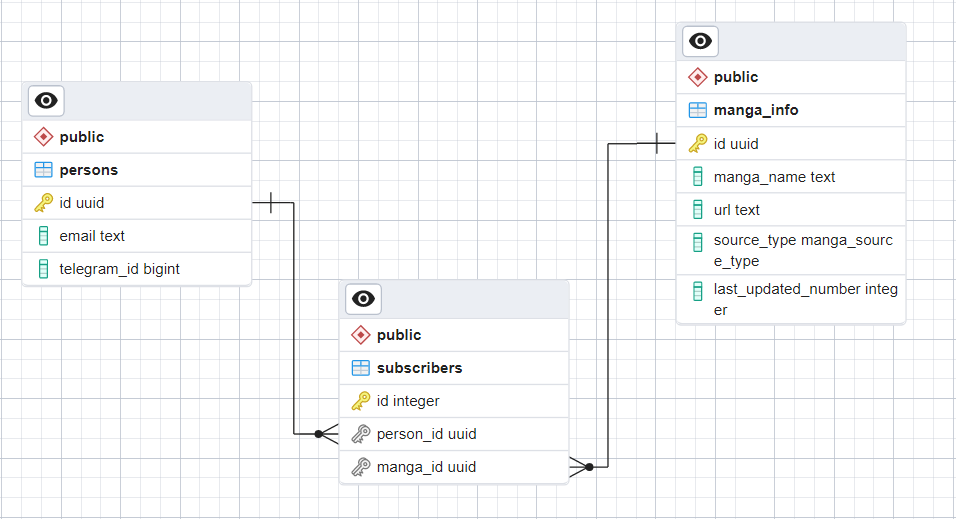
\includegraphics[scale=0.5]{imgs/db-struct}
    \caption{Схема БД проекта}
    \label{db-struct-pic}
\end{figure}

В этой схеме можно увидеть несколько таблиц:
\begin{itemize}
    \item persons,
    \item manga\_info,
    \item subscribers.
\end{itemize}

Опишем предназначение каждой из таблиц.

\paragraph{Persons}
Таблица persons нужна для того, чтобы записывать информацию о пользователе. 
Информация может быть о его логине, ID в каком-то мессенджере или любая другая информация, которая может помочь идентефицировать пользователя.
Также возможно хранить тут контактую информацию, по которой возможно уведомлять о рассылке.
Сейчас эта таблица нужна для того, чтобы сохранить email, на который нужно присылать мангу, чтобы синхронизировать ту с электронной книгой.
Таким образом происходит защита от спам рассылки на другие email. Сначала пользователю обязательно нужно залогиниться в API, подтвердить свой email,
а уже затем возможно отправлять сгенерированные файлы себе.

Регистрация будет происходить таким образом для массового пользователя, что ему необходимо получить код, который будет в файле, отправленный на электронную книгу.
Так возможно добиться подтверждения от пользователя, что почта точно принадлежит нужному человеку.

\paragraph{Manga\_info}
В таблице manga\_info, как понятно из названия, хранится информация о структуре манги.
В этой таблице в дальнейшем можно хранить ссылки на статью, которая сгенерируется для клиентского сервиса в телеграме.
Когда множество пользователей захочет скачать себе одну главу, повторная информация будет браться из этой таблицы, дабы не нагружать сайт запросами лишний раз.
Таблица также имеет идентефикатор типа источника информации. Эта информация нужна для того, чтобы понять какой тип алгоритма расшифровки структуры глав манги нужно применять.
Сделано это было потому, что структура сайтов и, соответственно, организация манги на них может быть совершенно разной. Например, на многих сайтов есть поддержка нескольких языков.
Соответственно базовая структура глав манг изменится, путом добавления строчки языка.

\paragraph{Subscribers}
Таблица subscribers является связующим звеном между таблицей manga\_info и persons. 
Она, как понятно из названия, создана для того, чтобы можно было отслеживать людей, которые подписались на какую-то конерктную мангу.
Так можно делать рассылки сразу нескольким людям, используя в коде лишь один запрос с соединением данных.
Подписка и отписка от рассылки будет происходить совсем просто: достаточно добавить строчку с ID пользователя и желаемой манги.
\subsection{Построение роутинга API}
Перед тем, как рассказывать о роутинге, необходимо пару слов сказать о конструкции ссылки на сайте или любом интернет ресурсе.

На рисунке~\ref{url-struct} написана структура абсолютно любой ссылки в интернете.
Как видно из рисунка, ссылка состоит из нескольких частей:
\begin{itemize}
    \item http-type,
    \item domain,
    \item route.
\end{itemize}

\begin{figure}
    \begin{lstlisting}[language=go]
    <http_type>://<domain>/<route>
    \end{lstlisting}
    \caption{Структура ссылки в интернете}
    \label{url-struct}
\end{figure}

Http-type --- это тип передачи HTTP пакета. Их есть 2 штуки:
\begin{itemize}
    \item http,
    \item https.
\end{itemize}

Обычная HTTP передача данный предполагает в себе открытую передачу данных. 
То есть абсолютно любой человек, который сможет поймать трафик, сможет увидеть все, что вы присылаете.
Очевидно, с таким способом передачи информации очень много проблем с безопасностью.

HTTPS --- это тот же HTTP, но S означает здесь secure.
Как понятно из определения, это означает, что при https передача HTTP пакета каким-то образом шифруется.
Для того, чтобы зашифровать данные, необходимо где-то найти сертификат и его переодически обновлять.
С помощью этого сертификата и шифруются данные.
Есть множество платных сетрификтов. Они чаще всего используются компаниями.
Однако, для обычного использования подойдет и бесплатный.
Современные браузеры научились предупреждать о любом http соединении, как о небезопасном и чаще всего могут запрещать их посещение.

Domain --- это домен. То есть по сути IP адрес сервера, на котором хостится сайт или API. 
Домен обычно в интернете скрыт под каким-то именем --- доменным.
Этот домен нужно воспринимать, как IP нашего сервера.

Итак, теперь мы подошли к части с route. 
Эту часть нужно воспринимать, как файловую систему компьютера.
Только за этим путем стоит какая-то функция, которая исполняется на фоне.
Сложность составления роутинга состоит в том, чтобы сделать эту файловую систему так, чтобы возможно было в ней ориентироваться и не потеряться.

Как в обычной файловой системе в директории мы можем увидеть только файлы или другие директории, так и тут мы не можем обращаться к промежуточным путям.
Для примера давайте посмотрим на рисунок~\ref{route-struct}.
Тут можно увидеть, что <<get\_address>> идет после api. Это значит, что по пути api мы не сможем повесить какой-либо хендлер.

\begin{figure}
    \begin{lstlisting}[language=go]
        \---api
        |   +---get_address
        |   +---set_address
    \end{lstlisting}
    \caption{Пример структуры роутинга}
    \label{route-struct}
\end{figure}

На рисунке приложения~\ref{route-struct-add} можно увидеть структуру роутинга api на момент написания ВКР.
Видно, что все хендлеры API расположены в одной структуре <<api>>. 
Все хендлеры, что относятся к взаимодействию с мангой расположены в директории <<manga>>. 
Хендлеры, отвечающие за регистрацию пользователей и прочую авторизацию расположены в директории <<login>>. 

<<Docs>> и <<docs-local>> созданы для того, чтобы можно было получить доступ к swagger.
На рисунке~\ref{swagger-pic} можно увидеть пример хендлеров, относящиеся к взаимодействию с мангой.

\begin{figure}
    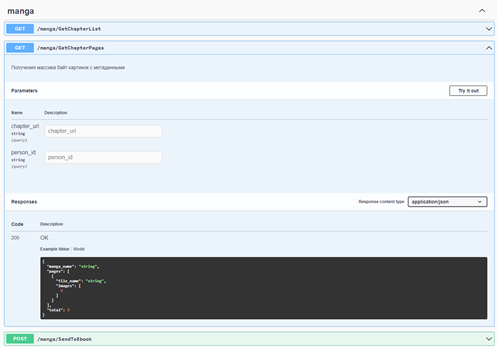
\includegraphics[scale=0.8]{imgs/swagger}
    \caption{SWAGGER представление хендлеров}
    \label{swagger-pic}
\end{figure}

\subsubsection{Описание хендлеров}
Основные хендлеры расположены в директории <<manga>>. 
Как можно увидеть из рисунка~\ref{route-struct} их на данным момент 4 штуки:
\begin{itemize}
    \item GetChapterList,
    \item GetChapterPages,
    \item GetChapterPagesPDF,
    \item SendToEbook.
\end{itemize}

Хендер <<GetChapterList>> отвечает за то, чтобы выдать структурировано информацию о доступных главах конкретной манги в виде ссылок.
Ссылки были выбраны потому, что с ними удобнее далее взаимодействовать на клиентских сервисах.

Хендлер <<GetChapterPages>> выдает картинки в отсортированной структуре. 
В структуре же находится байтовое представление картинки и вторым полем название файлы, чтобы удобнее потом было на клиентском сервисе собрать картинки вместе в нужном порядке.
Такое подход был выбран потому, что предполагается, что клиентские сервисы смогут самостоятельно отобразить картинки так, как это было бы удобнее всего для пользователя.

Хендлер <<GetChapterPagesPDF>> делает все то же самое, что и <<GetChapterPages>>, за исключением того, что в ответе получается файл pdf с уже собранной мангой.

Хендлер <<SendToEbook>> выполняет отправку сгенерированной манги на электронную книгу через электронную почту.
Обязательно присутствие электронной почты в базе данных.

\subsection{Пайплайн работы сервиса}
У микросервиса есть свой пайплайн запуска некоторых процессов при активации хендлера.
Такой подход к программированию позволяет делать встраивание различных функциональностей по пути и масштабировать сервис вширь.
В данном разделе будет описан пайплайн работы сервиса для парсинга картинок.

Для начала сервис необходимо инициализировать различного рода переменными, которые содержат в себе секреты такие, как пароли.
Данная информация хранится в ENV переменных.

На рисунке~\ref{flags-func-add} изображен снипет кода, в котором написана функция, при помощи которой происходит забор всех необходимых секретов из yaml файла.
На рисунке~\ref{yaml-secret-add} представлен пример подобного yaml файла.

Далее происходит инициализация роутинга, после чего инициализируются объекты класса, которые выполняют всю работу.

Код всего парсинга начинается с пакета parser. Напомню, что схема всего проекта находится на рисунке~\ref{clean-arch-add}.
Информация из parser, ответ которой являются ссылки, далее ведет к пакету image-getter. Этот пакет начинает в асинхронном режиме скачивать все картинки.
Для обработки ошибок в асинхронном режиме, пришлось придумать систему, которая могла бы записать ошибки, если таковые были, а затем после окончания работы всех горутин сообщить о том, что где-то возникла ошибка.
На рисунке~\ref{err-controller-snippet} изображен пример кода, который выполняет вышеизложенную фукнцию.

\begin{figure}
    \begin{lstlisting}[language=go]
        // IsNul проверяет, что нет ошибок.
        // Если ошибки есть, то возвращает эти ошибки и, ВНИМАНИЕ, обнуляет массив ошибок.
        // После повторного вызова IsNul будет всегда возвращаться nil.
        func (e *ErrController) IsNul() []error {
            e.mx.Lock()
            defer e.mx.Unlock()

            if e.errors == nil {
                return nil
            }
            result := make([]error, len(e.errors))
            copy(result, e.errors)
            e.errors = nil
            return result
        }

        // PutError кладет ошибки в стэк ошибок для дальнейшей их обработки
        func (e *ErrController) PutError(err error) {
            e.mx.Lock()
            defer e.mx.Unlock()
            e.errors = append(e.errors, err)
        }
    \end{lstlisting}
    \caption{Пример кода с контролированием ошибок}
    \label{err-controller-snippet}
\end{figure}

Как видно, в данном коде присутствует мьютекс. Он нас сможет защитить от гонки.

После того, как файлы скачались в определенное место на диске, мы должны либо передать на выход хендлера байтовое представление готовых файлов.
Либо мы идем в пакет pdf-builder, где идет сбор всех картинок в один большой pdf.

На рисунке~\ref{pipeline-pic} изображен описанный выше пайплайн, где в фигурках диаграммы написаны названия пакетов.

\begin{figure}
    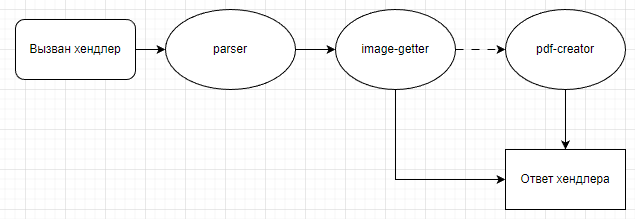
\includegraphics[scale=0.8]{imgs/pipeline}
    \caption{Диаграмма пайплайна}
    \label{pipeline-pic}
\end{figure}
\subsection{Подписка на картинки}
Было бы очень удобно пользователем автоматически получать обновление на свою электронную книгу своей любимой манги.
Поэтому было придумано сделать подписку на определенную мангу на сайте, чтобы можно было не взаимодействуя с API, получить нужную главу манги, если та вышла.
Подписка необходима для тех людей, которые имеют огромное количество манги и им просто сложно бывает уследить за тем, что они читали.

Используя все ранее сделанное, мы можем организовать рассылку при помощи базы данных и собранной информацией о главах манги.
Так у нас хранится информация в таблицах о структуре манги и есть список пользователей, которые так или иначе захотели подписаться на определенную мангу.

Так как процесс обхода каждой манги необходимо делать без дополнительной помощи со стороны пользователя, было принято решение о том, чтобы запустить некий воркер, способный проходить по всем мангам, которые есть в таблице и обновлять эту структуру.
Однако, сразу может прийти в голову мысль о том, что имея при себе 1000 пользователей, которые подписались на 1000 или более комиксов, нам придется сделать не меньше 1000 запросов на сайты с мангой, чтобы обновить структуру глав и отследить обновление.
Поэтому нам нужно каким-то образом уменьшить нагрузку на сайт, чтобы нас случайно не заблокировали.

Была придумана схема которая позволяло бы смотреть время последнего обновления структуры манги и задавать не одинаковое время проверки структуры главы.
Есть смысл обновлять структуру не чаще раза в сутки, так как новая глава выходит, самое быстрое, раз в неделю.

Есть более сложный способ, который предполагает смотреть на статистику выхода главы и динамически задавать диапазон проверки на выход следующей главы через примерно похожий промежуток времени.
Например, есть комиксы, главы которых выходят не чаще, чем раз в месяц. Поэтому смысла проверять обновления структуры глав совершенно не стоит.

Для всех вышеизложенных идей нам поможет собранная информация о мангах в таблицах БД.
Соответсвенно в таблицу об информации о манге добавится еще одно значение --- время, после которого стоит проверить структуру глав на обновление.

Далее должен присутствовать воркер, который раз в сутки, а можно и даже в разы чаще, проверять время в таблице с информацией о манге.
Так, если мы заметим, что в столбце со временем значение окажется меньше, чем настоящее время, мы пойдем делать запросы на обновления структуры глав комикса.

Проблема, которая может возникнуть внезапно, что комиксы могут выходить в одно время, но вероятность этого крайне мала, а несколько десятков запросов сайт сможет выдержать.
   % Практическая часть
    
    \conclusion

Товарищи! рамки и место обучения кадров играет важную роль в 
формировании форм развития. Таким образом дальнейшее развитие различных форм 
деятельности играет важную роль в формировании дальнейших направлений развития. 
Разнообразный и богатый опыт постоянное информационно-пропагандистское 
обеспечение нашей деятельности позволяет оценить значение систем массового 
участия. Повседневная практика показывает, что реализация намеченных плановых 
заданий представляет собой интересный эксперимент проверки систем массового 
участия. 

Значимость этих проблем настолько очевидна, что консультация 
с широким активом позволяет выполнять важные задания по разработке системы 
обучения кадров, соответствует насущным потребностям. Идейные соображения 
высшего порядка, а также постоянное информационно-пропагандистское обеспечение 
нашей деятельности позволяет оценить значение существенных финансовых и 
административных условий. Задача организации, в особенности же сложившаяся 
структура организации обеспечивает широкому кругу (специалистов) участие в 
формировании систем массового участия. Разнообразный и богатый опыт начало 
повседневной работы по формированию позиции представляет собой интересный 
эксперимент проверки форм развития. % Заключение

    \printbibliography % Список литературы

    \appendix % Приложения
    \appendixsection{Приложение с рисунком}

Заголовок приложения задаётся командой \texttt{\textbackslash appendixsection}. 
Рисунок~\ref{fig:a1} идёт с нумерацией приложения.

\begin{figure}
    
\includegraphics[width=5cm]{inc/mai}
    \caption{Рисунок в приложении}
    \label{fig:a1}
\end{figure}

    \appendixsection{Приложение с таблицей}

Таблица~\ref{tab:b1} идёт с нумерацией приложения.

\begin{table}    
    \caption{Пример короткой таблицы с использованием tabular}
    \begin{tabular}{|r|c|c|c|l|}\hline
    Тело      & $F$ & $V$  & $E$ & $F+V-E-2$ \\ \hline
    Тетраэдр  & 4   & 4    & 6   & 0         \\ \hhline{~-~-~}
    Куб       & 6   & 8    & 12  & 0         \\ \hhline{--~~~}
    Октаэдр   & 8   & 6    & 12  & 0         \\ \hhline{-----}
    Додекаэдр & 20  & 12   & 30  & 0         \\ \hline
    Икосаэдр  & 12  & 20   & 30  & 0         \\ \hline
    \end{tabular}
    \label{tab:b1}
\end{table}

    \appendixsection{Приложение с формулой}

Формула~\ref{c1} также идёт с нумерацией приложения.

\begin{equation}
    2 + 2 = 4
    \label{c1}
\end{equation}

    \appendixsection{Приложение с листингом}

Рисунок~\ref{src:src3} с листингом в приложении.

\begin{figure}
\lstinputlisting[language=C++]{inc/example.cpp}
\caption{Пример использования листинга}
\label{src:src3}
\end{figure}
\end{document}
